%% LyX 2.0.3 created this file.  For more info, see http://www.lyx.org/.
%% Do not edit unless you really know what you are doing.
\documentclass[twoside,english]{paper}
\usepackage{lmodern}
\renewcommand{\ttdefault}{lmodern}
\usepackage[T1]{fontenc}
\usepackage[latin9]{inputenc}
\usepackage[a4paper]{geometry}
\geometry{verbose,tmargin=3cm,bmargin=2.5cm,lmargin=2cm,rmargin=2cm}
\usepackage{color}
\usepackage{babel}
\usepackage{float}
\usepackage{bm}
\usepackage{amsthm}
\usepackage{amsmath}
\usepackage{amssymb}
\usepackage{graphicx}
\usepackage{esint}
\usepackage[unicode=true,pdfusetitle,
 bookmarks=true,bookmarksnumbered=false,bookmarksopen=false,
 breaklinks=false,pdfborder={0 0 0},backref=false,colorlinks=false]
 {hyperref}
\usepackage{breakurl}
\usepackage{makeidx}

\makeatletter

%%%%%%%%%%%%%%%%%%%%%%%%%%%%%% LyX specific LaTeX commands.
%% Because html converters don't know tabularnewline
\providecommand{\tabularnewline}{\\}

%%%%%%%%%%%%%%%%%%%%%%%%%%%%%% Textclass specific LaTeX commands.
\numberwithin{equation}{section}
\numberwithin{figure}{section}

%%%%%%%%%%%%%%%%%%%%%%%%%%%%%% User specified LaTeX commands.
\usepackage{babel}

\@ifundefined{showcaptionsetup}{}{%
 \PassOptionsToPackage{caption=false}{subfig}}
\usepackage{subfig}
\makeatother

\usepackage{listings}


\begin{document}

\title{Generalised parton distributions}

\author{Valerio Bertone}

\tableofcontents{}

\newpage
In this set of notes I collect the technical aspects concerning
generalised parton distributions (GPDs). Since the computation GPDs
introduces new kinds of convolution integrals, a strategy aimed at
optimising the numerics needs to be devised.

\section{Evolution equation}

In general, the evolution equation for GPDs reads:
\begin{equation}\label{eq:eveq}
\mu^2\frac{d}{d\mu^2}f(x,\xi) = \int_{-\infty}^{+\infty}\frac{dx'}{2\xi}V\left(\frac{x}{\xi},\frac{x'}{\xi}\right)f(x',\xi)\,.
\end{equation}
The GPD $f$ and the evolution kernel $V$ may in general be a vector
and a matrix in flavour space. For now we will just be concerned with
the integral in the r.h.s. of Eq.~(\ref{eq:eveq}) regardless of the
flavour structure. The support of the evolution kernel
$V\left(\frac{x}{\xi},\frac{x'}{\xi}\right)$ is shown in
Fig.~\ref{fig:GPDIntDomain}.
\begin{figure}[h]
  \begin{centering}
    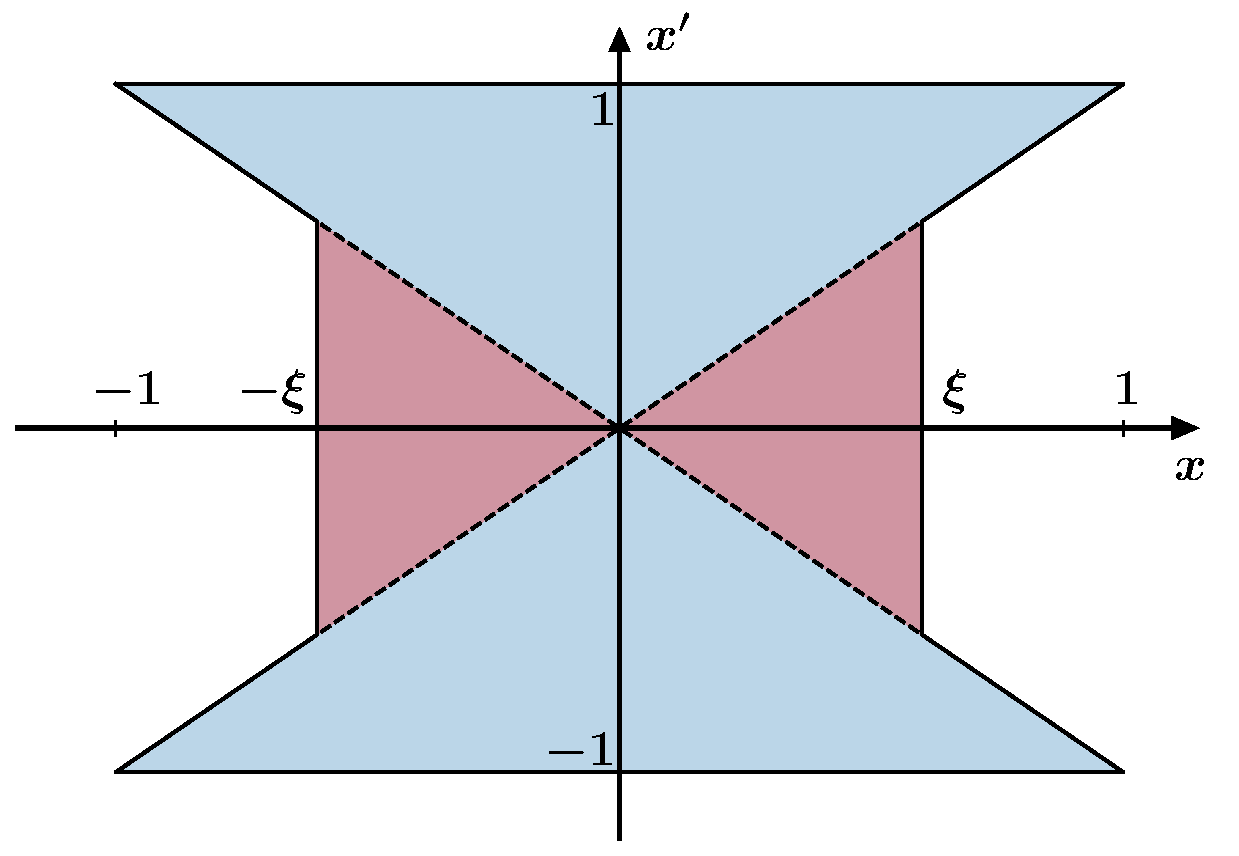
\includegraphics[width=0.7\textwidth]{plots/GPDIntDomain}
    \caption{Support domain of the evolution kernel
      $V\left(\frac{x}{\xi},\frac{x'}{\xi}\right)$.\label{fig:GPDIntDomain}}
  \end{centering}
\end{figure}
Without loss of generality, we can assume that $x>0$. Knowing the
support of the evolution kernel, Eq.~(\ref{eq:eveq}) can be split as
follows:
\begin{equation}\label{eq:eveq}
\begin{array}{rcl}
\displaystyle\mu^2\frac{d}{d\mu^2}f(\pm x,\xi) &=&\displaystyle
  \int_{x}^{1}\frac{dx'}{x'}\left[\frac{x'}{2\xi}V\left(\pm \frac{x}{\xi},\frac{x'}{\xi}\right)f(x',\xi)+\frac{x'}{2\xi}V\left(\mp \frac{x}{\xi},\frac{x'}{\xi}\right)f(-x',\xi)\right]\\
\\
&+&\displaystyle\theta\left(1-\frac{x}{\xi}\right)
  \int_{0}^{x}dx'\left[\frac{1}{2\xi}V\left(\pm \frac{x}{\xi},\frac{x'}{\xi}\right)f(x',\xi)+\frac{1}{2\xi}V\left(\mp \frac{x}{\xi},\frac{x'}{\xi}\right)f(-x',\xi)\right]\,.
\end{array}
\end{equation}
where we have used the symmetry property $V(y,y')=V(-y,-y')$. In the
unpolarised case, it is useful to define:\footnote{Notice the
  seemingly unusual fact that $f^{+}$ is defined as difference and
  $f^{-}$ as sum of GPDs computed at opposite values of $x$. This can
  be understood from the fact that, in the forward limit,
  $f(-x)= -\overline{f}(x)$, \textit{i.e.} the PDF of a quark computed
  at $-x$ equals the PDF of the corresponding antiquark computed at
  $x$ with opposite sign.}
\begin{equation}
\begin{array}{rcl}
\displaystyle f^{\pm}(x,\xi) &=&\displaystyle  f(x,\xi) \mp
                       f(-x,\xi)\,,\\
\\
\displaystyle V^{\pm}(y,y') &=&\displaystyle  V(y,y') \mp V(-y,y')\,,
\end{array}
\end{equation}
so that the evolution equation for $f^{\pm}$ can be split as:
\begin{equation}\label{eq:eveq2}
\begin{array}{rcl}
\displaystyle\mu^2\frac{d}{d\mu^2}f^{\pm}(x,\xi) &=&
  \displaystyle\int_{x}^{1}\frac{dx'}{x'}\frac{x'}{2\xi}
                                                         V^{\pm}\left(\frac{x}{\xi},\frac{x'}{\xi}\right)f^{\pm}(x',\xi)+\theta\left(1-\frac{x}{\xi}\right)
  \int_{0}^{x}dx'\frac{1}{2\xi}V^{\pm}\left(\frac{x}{\xi},\frac{x'}{\xi}\right)f^{\pm}(x',\xi)\\
\\
&=&\displaystyle I^{\pm,\rm DGLAP}(\xi,x)+I^{\pm,\rm ERBL}(\xi,x)\,.
\end{array}
\end{equation}
The first term in the second line of the equation above,
$I^{\pm,\rm DGLAP}$, corresponds to integrating over the blue regions in
Fig.~\ref{fig:GPDIntDomain}, while the second term, $I^{\pm,\rm ERBL}$,
results from the integration over the red regions. As indicated by the
subscripts, $I^{\pm,\rm DGLAP}$ and $I^{\pm,\rm ERBL}$ define the so-called
DGLAP and ERBL regions in $x$ relative $\xi$. Specifically, the
presence of the $\theta$-function in $I^{\pm,\rm ERBL}$ is such that for
$x>\xi$ this term drops leaving only the DGLAP-like term
$I^{\pm,\rm DGLAP}$. For $x\leq\xi$, instead, $I^{\pm,\rm ERBL}$ kicks in and
the evolution equation assumes the form of the so-called ERBL equation
that describes the evolution of meson distribution amplitudes
(DAs). Crucially, in the limits $\xi\rightarrow 0$ and
$\xi\rightarrow 1$ one should and does recover the DGLAP and ERBL
equations, respectively.

For convenience, we define the parameter:
\begin{equation}
\kappa = \frac{\xi}{x}\,,
\end{equation}
so that:
\begin{equation}
\frac{x'}{2\xi}
V^{\pm}\left(\frac{x}{\xi},\frac{x'}{\xi}\right)=\frac{1}{2\kappa}
\frac{x'}{x} V^{\pm}\left(\frac{1}{\kappa},\frac{1}{\kappa}
  \frac{x'}{x}\right)\equiv \mathcal{V}^{\pm}\left(\kappa,\frac{x}{x'}\right)\,,
\end{equation}
where the last equality effectively defines the function:
\begin{equation}
\mathcal{V}^{\pm}(\kappa,y) = \frac{1}{2\kappa y}
V^{\pm}\left(\frac{1}{\kappa},\frac{1}{\kappa y}\right)\,.
\end{equation}
Plugging this definition into the first integral in the r.h.s. of
Eq.~(\ref{eq:eveq2}) gives:
\begin{equation}
  I^{\pm,\rm DGLAP}(\xi,x)=\int_{x}^{1}\frac{dx'}{x'}\frac{x'}{2\xi}
                                                         V^{\pm}\left(\frac{x}{\xi},\frac{x'}{\xi}\right)f^{\pm}(x',\xi)=
                                                         \int_{x}^{1}\frac{dx'}{x'}\mathcal{V}^{\pm}\left(\kappa,\frac{x}{x'}\right)f^{\pm}(x',\xi)\equiv
                                                         \mathcal{V}^{\pm}\left(\kappa,x\right)\otimes
                                                         f^{\pm}(x,\xi)\,.
\end{equation}
Therefore, $I^{\pm,\rm DGLAP}$ has the form of a ``standard'' Mellin
convolution that, up to minor modifications due to the fact that
$\kappa$ depends on $x$, is easily handled by APFEL. Assuming a grid
in $x$ indexed by $\alpha$ or $\beta$, we have:
\begin{equation}
x_\beta I^{\pm,\rm DGLAP}(\xi, x_\beta) = \sum_\alpha \mathcal{V}_{\beta\alpha}^{\pm,\rm DGLAP}(\xi) f^\pm_\alpha (\xi)\,,
\end{equation}
with:
\begin{equation}
f^\pm_\alpha (\xi) = x_\alpha f^\pm(x_\alpha,\xi)\,,
\end{equation}
and:
\begin{equation}
\mathcal{V}_{\beta\alpha}^{\pm, \rm
  DGLAP}(\xi) = \int_{c}^{d}dx'\,\mathcal{V}^\pm\left(\kappa_\beta,x'\right)w_\alpha^{(k)}\left(\frac{x_\beta}{x'}\right)\,,
\end{equation}
where $\kappa_\beta=\xi/x_\beta$ and $\{w_\alpha^{(k)}\}$ is a set of
Lagrange interpolating functions of degree $k$ and the integration
bounds are:
\begin{equation}
  c=\mbox{max}(x_\beta,x_{\beta}/x_{\alpha+1})\quad\mbox{and}\quad c=\mbox{min}(1,x_{\beta}/x_{\alpha-k})\,.
\end{equation}

Now we need to treat $I^{\pm,\rm ERBL}$ in Eq.~(\ref{eq:eveq2}). The
structure of this term is rather unusual for APFEL because the
pre-computation of convolution integrals is usually done on
logarithmically-spaced grids in $x$ and integrating down to zero might
be problematic. However, contrary to forward distributions, GPDs are
generally well-behaved at $x=0$ and thus it is not strictly necessary
to reach this point in the integral.\footnote{We will verify this
  conjecture numerically.}  Upon this assumption, we find: to compute:
\begin{equation}
x_\beta I^{\pm,\rm ERBL}(\xi, x_\beta) = \sum_\alpha \mathcal{V}_{\beta\alpha}^{\pm,\rm ERBL}(\xi) f^{\pm}_\alpha (\xi)\,,
\end{equation}
with:
\begin{equation}
\mathcal{V}_{\beta\alpha}^{\pm, \rm
  ERBL}(\xi)=\theta\left(1-\frac{1}{\kappa_\beta}\right)\int_{\epsilon}^{x_\beta}dx'\,\frac{x_\beta}{x'^2}\mathcal{V}^\pm\left(\kappa_\beta,\frac{x_\beta}{x'}\right)w_\alpha^{(k)}(x')\,,
\end{equation}
where $\epsilon$ is a small number. Since the interpolating functions
$w_\alpha^{(k)}$ are such that:
\begin{equation}
w_\alpha^{(k)}(x)\neq0\quad\mbox{for}\quad x_{\alpha-k} <x<x_{\alpha+1}\,,
\end{equation}
the integral above can be computed more efficiently as:
\begin{equation}
  \mathcal{V}_{\beta\alpha}^{\pm,\rm
    ERBL}(\xi)=\theta\left(1-\frac{1}{\kappa_\beta}\right)\int_{a}^{b}dx'\,\frac{x_\beta}{x'^2}\mathcal{V}^\pm\left(\kappa_\beta,\frac{x_\beta}{x'}\right)w_\alpha^{(k)}(x')\,,
\end{equation}
with:
\begin{equation}
a = \mbox{max}(\epsilon,x_{\alpha-k})\quad\mbox{and}\quad b=\mbox{min}(x_\beta,x_{\alpha+1})\,.
\end{equation}

Finally, summing $I^{\pm,\rm DGLAP}$ and $I^{\pm,\rm ERBL}$ and multiplying by
a factor $x_\beta$, the evolution equation in Eq.~(\ref{eq:eveq}) can
be approximated on an grid in $x$ as:
\begin{equation}
\mu^2\frac{d}{d\mu^2}f^{\pm}_\beta(\xi) = \sum_{\alpha}\left[\mathcal{V}_{\beta\alpha}^{\pm,\rm DGLAP}(\xi)+\mathcal{V}_{\beta\alpha}^{\pm,\rm ERBL}(\xi)\right]f^{\pm}_\alpha(\xi)
\end{equation}
This is a system of coupled differential equation that can be solved
numerically using the fourth-order Runge-Kutta algorithm as
implemented in APFEL.

\section{Flavour structure}

In this section we report the leading-order (LO) evolution kernels
$\mathcal{V}^\pm$ taking into the flavour structure. The explicit
expressions of the relevant LO kernels are extracted from
Ref.~\cite{Blumlein:1999sc}.

The perturbative expansion of the evolution kernel is as usual:
\begin{equation}
V(x,x') = \sum_{n=0}^\infty \left(\frac{\alpha_s}{4\pi}\right)^{n+1}V^{(n)}(x,x')\,.
\end{equation}

\begin{equation}
\begin{array}{rcl}
\mathcal{V}^{(0)}(\kappa,y) &=&\displaystyle
                  2C_F\Bigg[\theta\left(\frac{1-y}{1+\kappa y}\right)
                  \theta\left(\frac{(1+\kappa)y}{1+\kappa y}\right)\mbox{sign}\left(\frac{1+\kappa y}{\kappa y}\right)
                  \frac{(1+\kappa)}{1+\kappa y}\left(\frac{1}{2\kappa}+\frac{y}{1-y}\right)\\
\\
&-&\displaystyle \theta\left(\frac{1-y}{1-\kappa y}\right)
                  \theta\left(\frac{(1-\kappa)y}{1-\kappa y}\right)\mbox{sign}\left(\frac{1-\kappa y}{\kappa y}\right)
                  \frac{(1-\kappa)}{1-\kappa y}\left(\frac{1}{2\kappa}-\frac{y}{1-y}\right)\Bigg]_+
\end{array}
\end{equation}

\newpage

\begin{thebibliography}{alp}

%\cite{Diehl:2003ny}
\bibitem{Diehl:2003ny}
  M.~Diehl,
  %``Generalized parton distributions,''
  Phys.\ Rept.\  {\bf 388} (2003) 41
  doi:10.1016/j.physrep.2003.08.002, 10.3204/DESY-THESIS-2003-018
  [hep-ph/0307382].
  %%CITATION = doi:10.1016/j.physrep.2003.08.002, 10.3204/DESY-THESIS-2003-018;%%
  %1016 citations counted in INSPIRE as of 30 Oct 2019

%\cite{Blumlein:1999sc}
\bibitem{Blumlein:1999sc}
  J.~Blumlein, B.~Geyer and D.~Robaschik,
  %``The Virtual Compton amplitude in the generalized Bjorken region: twist-2 contributions,''
  Nucl.\ Phys.\ B {\bf 560} (1999) 283
  doi:10.1016/S0550-3213(99)00418-6
  [hep-ph/9903520].
  %%CITATION = doi:10.1016/S0550-3213(99)00418-6;%%
  %86 citations counted in INSPIRE as of 13 Feb 2020


\end{thebibliography}




\end{document}
